{Given the graph of $f$, identify the intervals of increasing and decreasing as well as the $x$ coordinates of the relative extrema.\\
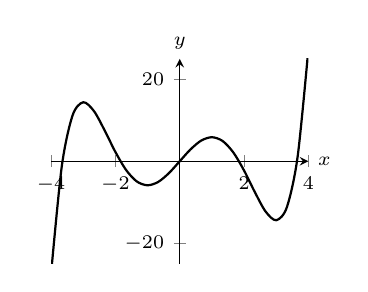
\begin{tikzpicture}
\begin{axis}[width=.4\textwidth,tick label style={font=\scriptsize },
	axis y line=middle,axis x line=middle,
    ymin=-25,ymax=25,
	xmin=-4,xmax=4,name=myplot]
\addplot [{\colorone},smooth,thick,domain=-4:4] {9*x-(10*x^3)/3+x^5/5};
\end{axis}
\node [right] at (myplot.right of origin) {\scriptsize $x$};
\node [above] at (myplot.above origin) {\scriptsize $y$};
\end{tikzpicture}}
{decreasing on $(-3,-1)\cup(1,3)$,\\
increasing on $(-\infty,-3)\cup(-1,1)\cup(3,\infty)$;\\
local maxima when $x=-3,1$,\\
local minima when $x=-1,3$.}
